\question A thin, uniformly charged rod of length $L$ carrying total charge $Q$ lies on the $x-$axis, centered on the origin. 
\begin{parts}
\part\label{integral} Neglecting the thickness of the rod, write an expression for the electric field $\efield$ of the rod at a point along its central axis (the $y-$axis). You may leave your expression in integral form.

\begin{center}
	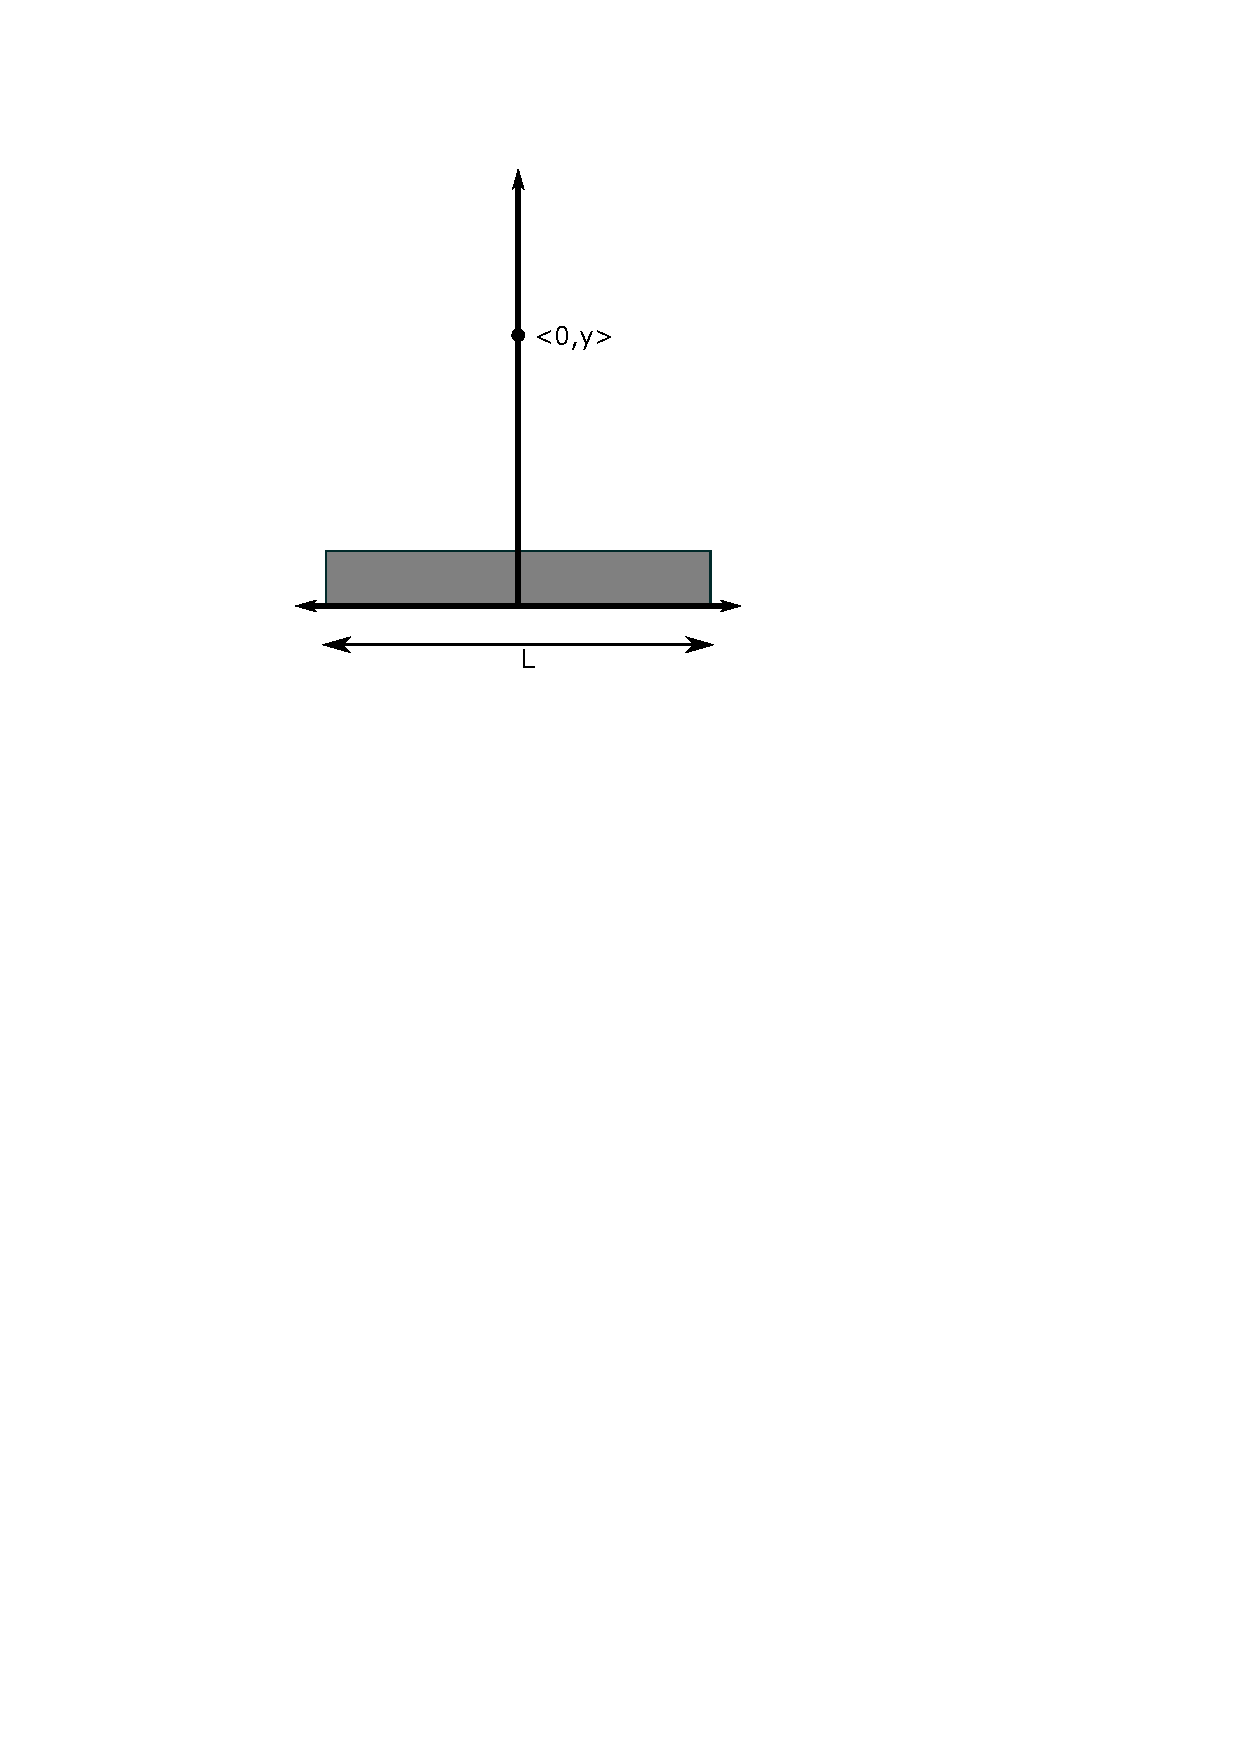
\includegraphics[width=5cm]{problem3a.pdf}
\end{center}

\newcommand{\length}{4 cm}
\newcommand{\Q}{$6\ \mu\text{C}$}
%\vspace{5cm}
\newpage
	\part If your expression from part (\ref{integral}) is correct, the integral evaluates to 
	\begin{equation*}
		\efield = \frac{1}{4\pi\epsilon_0}\left[\frac{Q}{y\sqrt{y^2+(L/2)^2}}\right]\hat{y}
	\end{equation*}
	 Where $y$ is the vector pointing from the center of the rod to a point along its  perpendicular axis.
	 
	 Use this information to answer the following question:
	 
	 Two thin, uniformly charged rods, both with length $L=$\length{} and charge $Q=$\Q, have their ends at the origin and lie perpendicular to one another as shown in the figure. What is the force $\vec{F}$ on a proton placed at the point $<L/2,-L/2>$ (the intersection of the axes of the rods)?
\begin{center}
	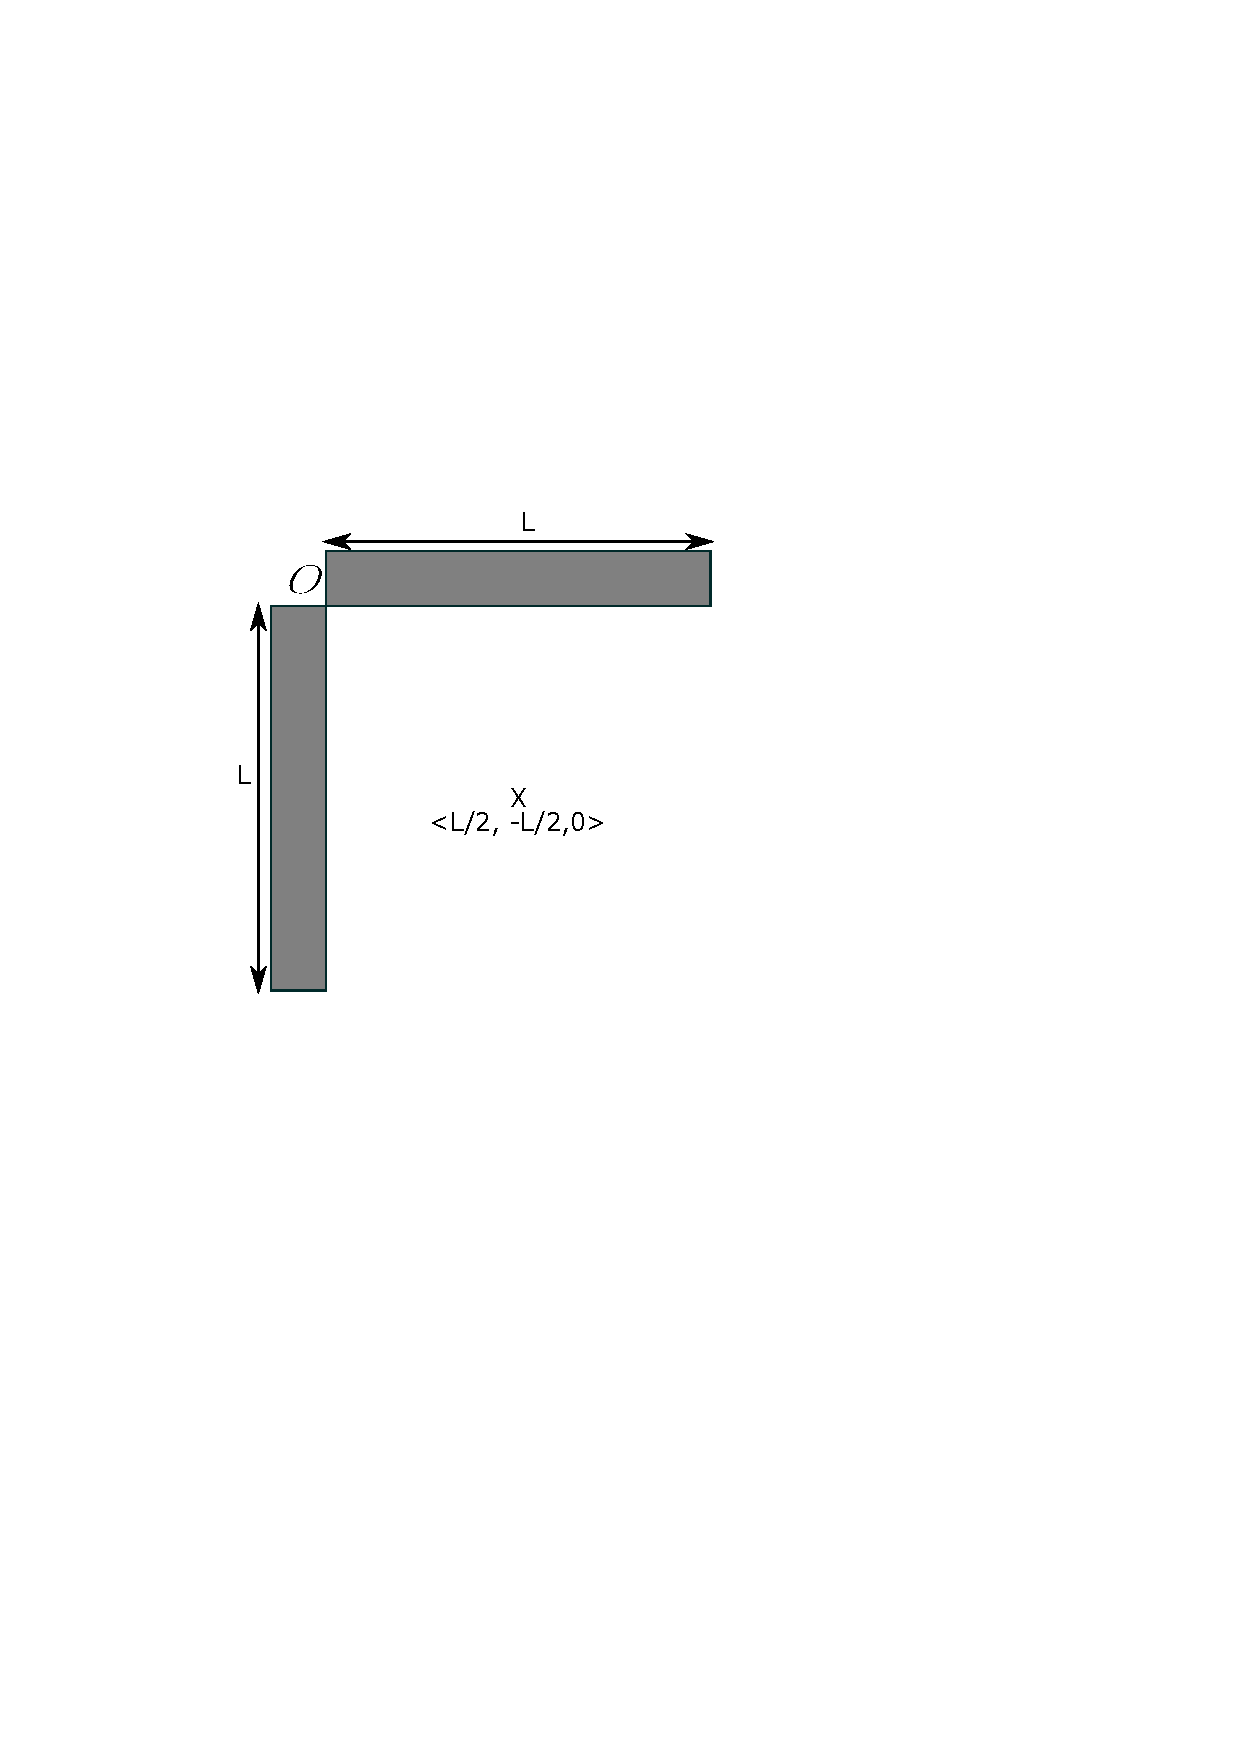
\includegraphics[width=5cm]{problem3.pdf}
\end{center}

\end{parts}